\documentclass[12pt]{article}


\usepackage{multicol}
\usepackage[numbers]{natbib}
\usepackage{pdfpages}

\usepackage{url}
\usepackage{graphicx}


\setlength{\hoffset}{0pt}
\setlength{\voffset}{0pt}
\setlength{\oddsidemargin}{0pt}
\setlength{\topmargin}{0pt}
\setlength{\topsep}{0pt}
\setlength{\headsep}{0pt}
\setlength{\headheight}{0pt}
\setlength{\textwidth}{6.5in}
\setlength{\textheight}{9in}
\setlength{\parskip}{11pt}
\setlength{\parindent}{0pt}

% \newcommand{\solutionname}{[Solution Name]}
\newcommand{\organization}{TeMa}
\newcommand{\solutiontitle}{Modification and Use of Synthea to Account for Patient Vaccination Choice}
\newcommand{\challengecategory}{I (Enhancement to Synthea)}
\newcommand{\ABSTRACT}{
	Recent trends have shown an increase in the number of parents that request non-medical exemptions (NMEs) to routine pediatric vaccinations \cite{latimes-antivax,antivax}.  The resulting decline in childhood vaccinations has led to increases in childhood disease outbreaks \cite{antivax-data}.  In its current form, Synthea \cite{synthea} does not account for these variations in pediatric vaccinations \cite[p. 15]{challenge-webinar-slides}, which are the result of patient health care preferences that do not align with accepted optimal approaches to health care.  
    For this effort, we modify the existing immunization workflow in Synthea so that it accounts for patient preferences and produces synthetic health records (or synthetic patients) with a more varied vaccination history, specifically with respect to the Measles, Mumps, and Rubella (MMR) vaccine.  We demonstrate the utility of this modification by developing a prototype module for childhood measles that is responsive to whether the patient has received the MMR vaccination.  To validate the results, we use linear regression to compare the synthetic data produced to existing public vaccination estimates \cite{antivax-data}.  Finally, we comment on how this development enhances the capability of Synthea and propose multiple avenues for future research efforts that, using this capability, could have significant impacts on public health and facilitate Patient Centered Outcomes Research (PCOR).
}





\begin{document}

%%% COVER PAGE

\thispagestyle{empty}

~
\vspace{\stretch{1}}

\begin{center}
    {\huge \solutiontitle} \\[24pt]
    {\Large Submission for the Synthetic Health Data Challenge} \\[24pt]
    {\Large By:} \\[24pt]
\end{center}

\begin{multicols}{2}
\begin{center}
	Michael D. Teter\\
	miketeter@yahoo.com
\end{center}

\columnbreak

\begin{center}
    Christopher E. Marks\\
    cemarks@alum.mit.edu
\end{center}
\end{multicols}

\vspace{\stretch{0.2}}


\noindent \textbf{Challenge Category:} \challengecategory
\\

\vspace{\stretch{1}}

\clearpage


%% Body %%

\setcounter{page}{1}

\begin{center}
    {\LARGE \solutiontitle}
    \\[11pt]
    \begin{minipage}{0.9\textwidth}
      \textbf{Abstract:}
      \ABSTRACT
    \end{minipage}
\end{center}

\noindent \textbf{Github:} \url{https://github.com/teterholdings/Synthea_NME}\\
\noindent \textbf{YouTube:} \url{https://youtu.be/BVlPj1qW75w}
  
\section{Overview}

One of the known limitations of Synthea is that it does not allow for variation in care trajectories \cite[p. 15]{challenge-webinar-slides}.  This limitation is significant in the context of the Office of the National Coordinator (ONC) objective of enabling Patient-Centered Outcomes Research (PCOR) \cite[pp. 3,9]{challenge-webinar-slides}, as it does not account for individual patient preferences or objectives in applying treatments.  One area where patient preferences are rapidly changing, and that could have serious consequences on public health, is in the area of vaccinations \cite{antivax,vaccine-rates-cdc}.  Additionally, many US states have permissive non-medical exemption policies, which make it relatively easy for parents to decline routine vaccinations for their children.

In this effort, we modify Synthea software to account for parent non-medical exemption decisions for their children.  We create a prototype ``Measles'' module that takes advantage of this code modification, omitting the MMR vaccine from some patients' records and making these patients susceptible to measles infection.  These updates make it possible to analyze where there might be high-risk regions for measles in the US, and investigate what-if scenarios based on different assumptions about NME rates in the future.

While our use-case is focused on pediatric vaccination, our work also has particular relevance to COVID-19 vaccination in the United States.  Because this vaccine is elective, and also as a result of political polarization, a large portion of the population has not received it \cite{latimes-antivax}.  The methods and results we present could be applied to COVID-19 and other vaccinations to analyze the effects of different vaccination rates in order to predict medical resource requirements, educate the public, and inform public policy decisions.

\section{Methods}

To prototype the non-medical exemption capability, we modified the immunizations module \cite{synthea-immunizations} workflow in Synthea to look for a patient NME attribute before adding the immunization to the patient's record.  For example, before administering an MMR vaccine, the software first checks for an attribute called ``\texttt{mmr NME}.''  If this patient attribute exists, the MMR workflow is skipped and the MMR record is omitted from the patient's records.

This small change in the Immunizations module enables a user to write drop-in JavaScript Object Notation (JSON) modules that set NME attributes for patients, resulting in an unvaccinated subset of the population.  Like any other modules, these modules can be called at runtime or compiled into Synthea.  

We created the \texttt{measles.json} module depicted in Figure \ref{fig: measles.json} \cite{synthea-module-builder} to apply this new capability.  The module uses the lookup table transition capability, developed recently to facilitate COVID-19 modeling, to apply NME rates that vary over geographic region and time.  We set the default NME rate at or below the national average (in Figure \ref{fig: measles.json} it is 1.86\%, the national average), using the lookup tables to incorporate NME rates information in US states for periods where this data is publicly available \cite{vaccine-exemptions-cdc}.

\begin{figure}[!hbt]\centering
    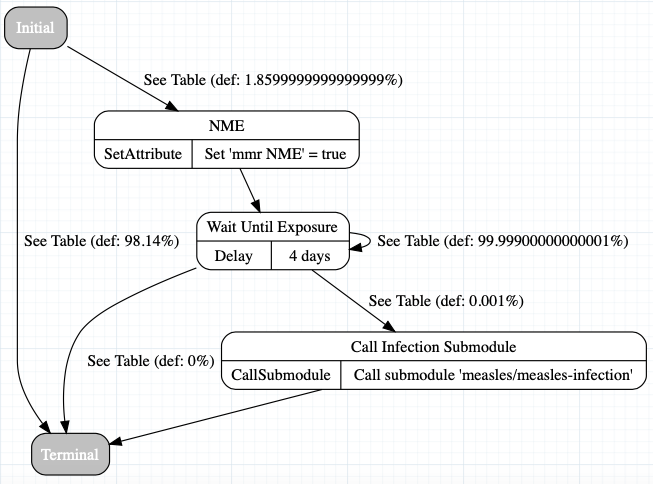
\includegraphics[width=0.8\textwidth]{figures/measles_json.png}
    \caption{Measles NME module (\texttt{measles.json}). \label{fig: measles.json}}
\end{figure}

If a patient has an NME, then the patient is susceptible to measles infection.  Once again, we use a lookup table transition to call the measles infection submodule for a subset of these patients, using workflow based on the existing Synthea COVID-19 modules.  As depicted in Figure \ref{fig: measles.json}, these patients loop through the ``Wait Until Exposure'' state in four-day increments until they either are exposed to measles or terminate the module.  We designed the measles exposure lookup table for this simulation state transition to loosely track with measles infection rates in the United States over the past 10 years \cite{measles-cases-cdc}.  The default transition probabilities include a very small probability that the patient will be exposed to measles; otherwise the patient continues to cycle through the ``Wait Until Exposure'' state.  

If a patient is exposed, the patient transitions to the ``Call Infection Submodule'' state, which executes the measles infection workflow (not depicted). %%(Figure \ref{fig: measles-infection.json}).
This workflow is based on the COVID-19 infection submodule, progressing through common measles symptoms and, in some cases, hospitalization and/or death.  

% \begin{figure}[!hbt]\centering
%     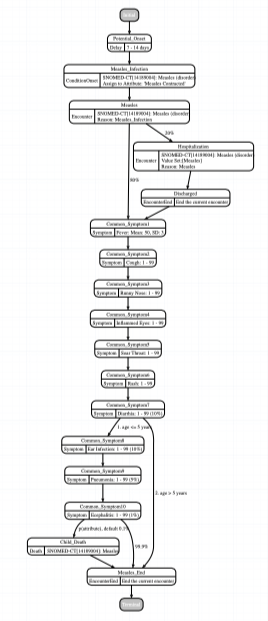
\includegraphics[width=0.5\textwidth]{figures/measles-infection_json.png}
%     \caption{Measles infection submodule (\texttt{measles/measles-infection.json}). \label{fig: measles-infection.json}}
% \end{figure}

\section{Results and Validation}

The Center for Disease Control (CDC) provides vaccine non-medical exemption rates by state for recent years \cite{vaccine-exemptions-cdc}, which we used to tailor the NME transition probabilities as discussed in the previous section.  These same statistics can be used to validate the NME rates in the data in Synthea.  For our implementation, we aim to ensure that synthetic NME rates and measles infection rates are approximately proportional to known data.

\begin{figure}[!htb]\centering
    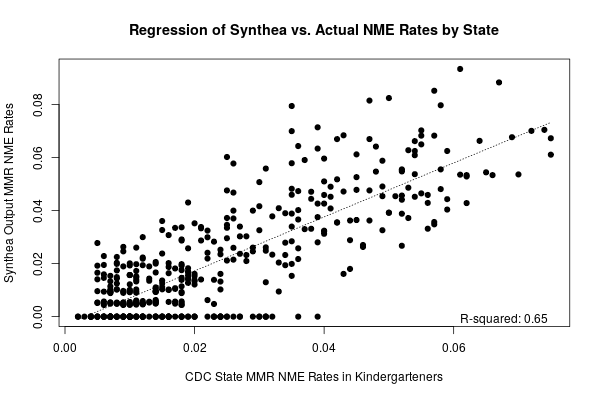
\includegraphics[width=0.8\textwidth]{figures/nme_states_reg.png}
    \caption{Regression of synthetic data NME rates against known NME rates in the US. \label{fig: nme-state-regression}}
\end{figure}


We generated approximately 5000 synthetic health records for each US state using our modified Synthea immunization and measles modules.  In order to focus on the population that might have NMEs, we limited the record generation to patients ages 6-30.  We then compared the rate of NMEs in kindergarten-aged children per state, per year against the known data points in the \citet{vaccine-exemptions-cdc} data.  We found that the NME rates in the synthetic data correlated with the actual NME rates (correlation coefficient: 0.81, $R^{2}$: 0.65).  This result validates that our implementation is producing more records with NMEs for locations and times where and when there are more people with NMEs in the United States.  Figure \ref{fig: nme-state-regression} provides a scatter plot with the regression line and $R^{2}$ value for this analysis. 

Using these same 5000 synthetic health records, we examined the measles infection rates and again compared against known measles infections data from the Center for Disease Control \cite{measles-cases-cdc}.  Figure \ref{fig: measles-cases-comparison} shows bar plots of measles infection rates in the United States from (a) the synthetic (Synthea-generated) data, and (b) CDC monitoring.  The synthetic measles infection rates track proportionately with observed infection rates.   

\begin{figure}[!hbt]\centering
    \begin{tabular}{cc}
    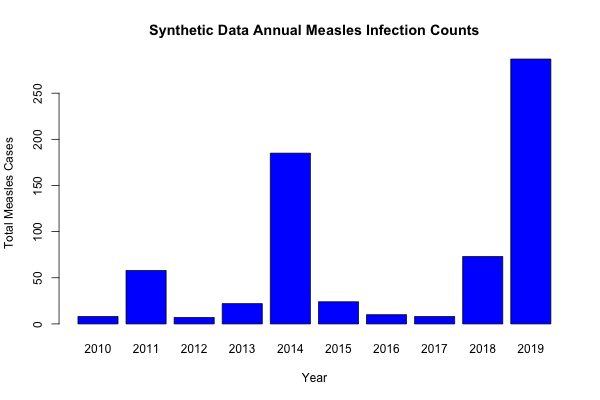
\includegraphics[width=0.45\textwidth]{figures/measles-annual-counts.png} &
    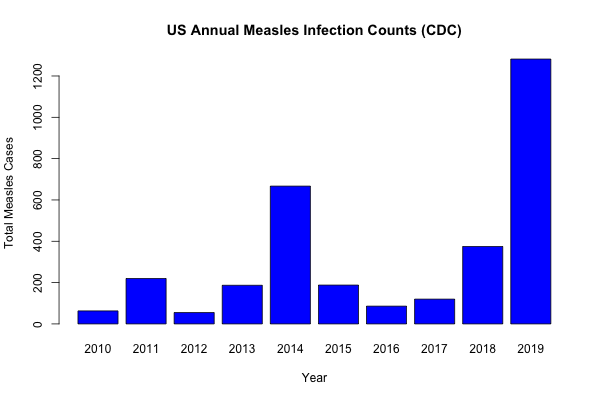
\includegraphics[width=0.45\textwidth]{figures/cdc-measles-annual-counts.png} \\
    (a) Synthetic measles rates. & (b) CDC measles rates.
    \end{tabular}
    \caption{Comparison of measles infection rates in synthetic and CDC data.\label{fig: measles-cases-comparison}}
\end{figure}

The synthetic output can also be spatially compared to known measles incidence.  Figure \ref{fig: map-comparison} provides a density map of the 2019 US measles outbreak \cite{cdc-measles-increases}, along with a heat map of all of the Synthea-generated measles cases.  A qualitative comparison of the two maps shows some similarities and some differences.  Consistencies between the two plots result from the infections occurring in population centers where NME rates are high, most notably in the northeast and northwest.  Discrepancies are inevitable; other than preferring populated areas for measles infections, we did not make an effort to geographically match known outbreaks.  What is important is the qualitative similarity between the two maps: each as a few places with large numbers of cases, a more substantial number of places with low infection counts, and a large portion of the country (north \& central states) with very few or zero infections.  

\begin{figure}[!hbt]\centering
    \begin{tabular}{cc}
        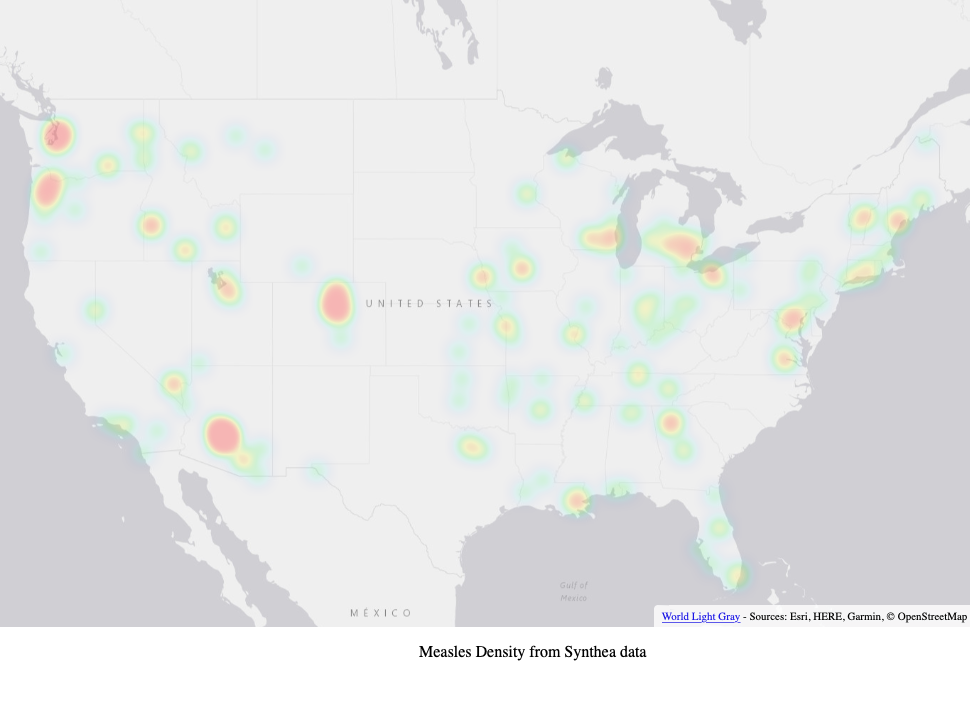
\includegraphics[width=0.45\textwidth]{figures/synthea-measles-density-gray.png} &
        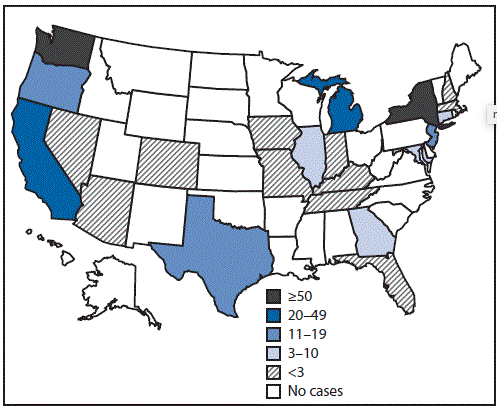
\includegraphics[width=0.45\textwidth]{figures/cdc-measles-density.png} \\
        (a) Synthea-generated measles density across US. &
        (b) CDC map of 2019 US measles density
    \end{tabular}
    \caption{Comparison of 2019 US measles outbreaks with Synthea output. \label{fig: map-comparison}}
\end{figure}

Varying the lookup tables naturally produced different results.  Lower probabilities, including a lower default NME probability in the measles module (Figure \ref{fig: measles.json}), combined with larger sets of generated records tended to produce results that performed better in our qualitative and quantitative validation checks.  This result is not surprising; NMEs and measles are low-density events.  To study them in that context one needs a large statistical population.  In most of our test cases, we generated 1000-5000 records per state.  In order to obtain useful rates of NMEs and measles infections from these relatively small sets of records, we set probabilities that were higher than observed rates in the US.  While these probabilities had the intended effect of boosting the number of measles cases, they had the unintended effect of introducing ``herd immunity,'' which ended up inhibiting our ability to model subsequent infections.

\section{Implementation Details}

We cloned the Synthea source code from github \cite{synthea-github}, made the changes described in the preceding sections, and recompiled into a ``jar'' with dependencies to execute.  We found that, although we could drop in the measles module and measles-infection submodule, we could not get Synthea to load lookup tables from a local path at runtime.  Therefore, we put our prototype modules and lookup tables in the source code so that the \texttt{synthea-with-dependencies.jar} contained all of our work.  The code, along with documentation of the steps we followed is on github at \url{https://github.com/teterholdings/Synthea_NME}.

\section{Utility}

The very concept of accounting for the patient's preferences and health objectives is fundamental to PCOR \cite{pcori}.  In its current state, Synthea does not account for these preferences, which can result in patient records that are not representative of the population.  By capturing one such patient preference, childhood MMR vaccine NMEs, we have provided a method for incorporation of more diversity in synthetic data generation that will enable researchers to more directly investigate and optimize patient-centered outcomes.  

The synthetic patient records generated by our prototype include non-medical MMR exemptions for some patients and, consistent with recent findings (see, e.g., \cite{arvil-vaccine-exemptions}), reflect a corresponding increase in childhood measles in the US.  These modifications to Synthea can be useful in analyzing the impacts of non-medical exemptions to vaccines.  Our current, prototype implementation includes workflows in which patients are hospitalized, or die from measles.  This prototype can be used immediately to compare the costs, in terms of hospitalizations and deaths, of different NME scenarios in the US.

The outputs of the simulation under different scenarios would be valuable in informing public policy decisions for NMEs, as well as for educating the public.  It would be very useful, for example, to understand and to be able to compare the costs of NMEs for different vaccines, in order to make informed decisions on which vaccines might be ``negotiable,'' and which are not.  More detail in the infection submodule, e.g., inclusion of additional long term effects of childhood measles, would increase the utility of these NME cost analyses.  Finally, this synthetic data would be very useful in projecting medical resource and care requirements, especially with respect to pediatrics and complex care, in the most likely future scenarios.

\clearpage

%% References

\bibliography{refs}
\bibliographystyle{plainnat}

%% Registration Form

%% \includepdf[pages=-]{registration_form.pdf}

\end{document}
